\chapter{Métodos}

A todas as experiências foram aplicadas as métricas apresentadas, excepto no benchmark onde teríamos métricas de comparação a ele próprio.\par
Para a escolha de melhor modelo dentro das experiências foi escolhido o modelo que melhor resultados apresentou para a métrica em questão. Sendo esta o GPD $Norm^{2}$ enquanto não encontramos uma melhoria tanto na alocação em falta como na em demasia, ao que se seguida foi usado o GPD Positivo.\par
No caso das Redes Neuronais a hiper parametrização foi feita também deste modo, sendo que primeiro se encontrou uma hiper parametrização adequada aos dados, usando uma arquitetura simples e só depois com essa configuração foi feita a experiência  nas várias arquiteturas.\par
O objectivo é conseguir um modelo que tenha a uma Alocação Total em Falta e Alocação Total em Demasia menor que o Benchmark, dentro dos anos 2019 a 2022. Logo em termos de métricas um GPD Positivo mais elevado possível.\par

\thispagestyle{plain}
\section{Estatisticos}

Em estatística conseguimos encontrar vários métodos de estudo de séries temporais. Estes métodos são normalmente usados como primeira abordagem para fazer previsões.\par
Estes modelos podem ser \gls{AR}, onde vão fazer previsões baseados num número \textit{(p)} de dados anteriores. Estes modelos são construídos com a noção de que um valor é linearmente dependente de \textit{p} valores anteriores numa série temporal.\par

\begin{alignat*}{2} 
    & X_{t} : \text{Valor no } t \text{ a prever.} &\quad& p : \text{O número observaçoes anteriores.} \\
    & \varphi_{i} : \text{Coeficiente na observação } i. &\quad& q : \text{O número observaçoes anteriores.} \\
    & \epsilon_{i} : \text{Erro na observação } i. &\quad& \theta_{i} : \text{Coeficiente na observação } i \text{.} \\ 
    & \mu : \text{Média dos valores } X \text{.} 
\end{alignat*}

\bigskip
\gls{AR} \\

\begin{equation} \label{eq:ar} 
    X_{t} = \sum_{i=1}^{p}\varphi_{i} X_{t-i} 
\end{equation}
\smallskip

Outra família destes modelos são os de \gls{MA}, onde a média de um número de observações \textit{(q)} em conjunto com os erros \textit{($\epsilon$)} e os coeficientes \textit{($\theta$)} é usada para prever os valores seguintes.\par
\bigskip
\gls{MA} \\

\begin{equation} \label{eq:ma} 
    X_{t} = \mu + \sum_{i=1}^{q}(\theta_{i} \epsilon_{t-i}) + \epsilon_{t}
\end{equation}
\smallskip
Estes dois tipos de modelos podem ser juntos criando os modelos \gls{ARMA}. que junta as capacidades dos modelos anteriores.\par

\bigskip
\gls{ARMA} \\

\begin{equation} \label{eq:arma} 
    X_{t} = \sum_{i=1}^{p}\varphi_{i} X_{t-i}  + \mu + \sum_{i=1}^{q}(\theta_{i} \epsilon_{t-i}) + \epsilon_{t}
\end{equation}
\smallskip

Existem mais modelos de previsão estatística baseados nestes com algumas variações, mas para este trabalho, e apenas como ponto de comparação às redes neuronais, ficamos apenas por estes.\par
As variáveis em estudo por tipo de modelo foram retiradas das autocorrelações temporais usando os métodos de sugestão da ferramenta \hyperref[se:muaddib]{MuadDib}:\\


\begin{table}[h] \centering
\begin{tabular}{lrrrr}
    \toprule
     & p & q \\
    \midrule
    \gls{AR} & 1/ 2 / 23 / 24 / 25 / 48 / 144 / 168 / 192 / 336 & NA \\
    \gls{MA} & NA & 1 / 24 \\
    \gls{ARMA} & 1 & 1 \\
    \bottomrule
    \end{tabular}
    \label{tab:varsstats} 
    \caption{Variáveis de estudo dos modelos AR/MA}
\end{table}


Todos estes modelos foram testados usando o software disponível na package de python \href{https://www.statsmodels.org/stable/index.html}{statsmodel}, com a classe \href{https://www.statsmodels.org/stable/generated/statsmodels.tsa.arima.model.ARIMA.html}{ARIMA}.
 \label{se:metstats}


\newpage
\thispagestyle{plain}
\section{Redes Neuronais}

As redes neuronais podem ser descritas como uma função desconhecida \textit{f(x)=y} onde durante o treino a função \textit{f} é criada através da manipulação dos pesos da sua arquitetura usando os dados de treino, x, de forma a diminuir ao máximo uma função de perda . Sendo \textit{f'(x)=y'} um modelo já treinado onde \textit{y'} é a previsão, a função de perda \textit{fp(y, y')} idealmente igual a 0, com \textit{y'=y.}\\
Neste trabalho o \textit{x} são todos os dados apresentados no capitulo \hyperref[ch:estudo_2]{Estudo 2}, em grupos de 128 (horas), e o \textit{y} é a energia usada, "UpwardUsedSecondaryReserveEnergy" no modelo de previsão de energia a subir e "DownwardUsedSecondaryReserveEnergy" no modelo de previsão de energia a descer, nas 24 horas subsequentes. A \textit{fp} é um dos factores de estudo, assim como outros parâmetros dentro das arquiteturas de modelos, \textit{f}.\\
Assim utilizamos os 168 horas (1 semana) para prever as 24 horas seguintes. As 24 horas seguintes são o objectivo do estudo, energia a alocar no dia seguinte. As 168 horas são escolhidas graças às \hyperref[tab:tempcorr]{maiores autocorrelações temporais}, de onde as maiores fora das primeiro 48 horas são 144, 168, 192 horas ou seja, 6, 7 e 8 dias respectivamente, onde em ambos os casos 7 dias era o valor com maior correlação.\\
As condições em estudo são feitas através da ferramenta \hyperref[se:muaddib]{MuadDib}, seguindo vários percursos entre as combinações possíveis, de modo a conseguir a combinação óptima, maior GPD Positivo.\\


\subsection{Arquitecturas}

\gls{FCNN}, \gls{CNN} , RNN são as arquitecturas mais simples que vamos estudar. Estas vão apenas pegar nos blocos e vamos criar as mesmas "Vanila" e "Stacked" com 2 blocos (ex: StackedCNN) ou 6 blocos (ex: Stacked6CNN).\\
UNET, \gls{LSTM} são arquiteturas mais complexas e pesadas. Como descrito anteriormente uma mais utilizada em análise de imagens, e outra em análise de texto respectivamente.\\
Transformers são as mais pesadas qualidade comum da família de "generative AI".

\subsection{Função de Perda}

Nos primeiros testes mais simples foi imediato a discrepância entre os erros da energia alocada em demasia e em falta. Sendo que estes erros estão em dimensões completamente diferentes.
\begin{figure}[H]
    \centering
    \includegraphics[width=\textwidth]{plots/allocs_results_shadow.png}
    \caption{Resultados de alocações totais em diferentes arquiteturas}
    \label{fig:resexparchs}
  \end{figure}

Na energia em falta, estamos a lidar com valores na dimensão de $10^{6}$ nos resultados, sendo que o benchmark está nos $10^{5}$. Logo estão bastante acima do que queremos. Por outro lado na Energia em Demasia temos resultados na ordem dos $10^{6}$ e o benchmark está na ordem dos $10^{7}$. Isto dá-nos espaço para aumentar os resultados da Energia em Demasia mantendo-os ainda abaixo do benchmark para diminuir os resultados da Energia em Falta com objectivo de a ter também abaixo do benchmark.\\
Para combater esta desigualdade foram criadas várias funções de perda para atribuir melhor peso a ambas de modo a atingir melhor o objectivo geral.\\
De maneira que partimos esta experiência em duas partes. A primeira parte, Função de Perda Avançada, vai estudar diferentes maneiras de distribuir pesos entre a energia alocada em demasia e a em falta. A segunda vai escolher qual a melhor função de perda a aplicar nessa distribuição de pesos, ou vice-versa.\\


\subsubsection{Funções de Perda}
Depois de escolhidos os pesos nos diferentes grupos são testadas as funções a aplicar. Aqui vamos manter simples e testar apenas as mais comuns em problemas de regressão linear: \gls{MAE}, \gls{MSE}, \gls{MSLE}.\\
\gls{MAE} é usada no geral em problemas em que os dados têm um histograma linear, e um erro normalmente distribuído.\\
\gls{MSE} é usado para atribuir maior peso aos erros maiores, do que no \gls{MAE}. Fazendo com que o modelo se concentre mais em aprender a diminuir erros maiores.\\
\gls{MSLE} é sugerido em dados que têm uma histograma exponencial.\\

% TODO: meter formulas? depende do espaço


\subsubsection{Função de Perda Avançada}\label{se:advancedloss}

Para escolher a melhor maneira de distribuir pesos foi criada uma função de perda com diferentes regras, que distribuem o peso da amostra.\\
\href{https://github.com/alquimodelia/alquitable/blob/main/alquitable/advanced_losses.py#L33}{Mirror Weights (Pesos Espelhados)}\\
Que vai distribuir os pesos da amostra consoante um rácio predefinido e o próprio erro da amostra.\\
Os pesos nas amostras vão ser divididos entre os erros negativos (alocação em demasia) e os positivos (alocação em falta). Consoante uma variável lógica,  uns terão peso 1 e os outros serão o próprio erro em absoluto. Dando assim um peso equivalente ao erro, quanto maior o erro maior o peso da amostra na função de perda, do lado da amostra escolhido (em demasia ou em falta).\\
Pode ser multiplicado um rácio tanto a um dos pesos como a outro, sendo estes rácios que irão equilibrar as diferenças entre a alocação em falta e a em demasia. E o sinal do rácio influencia qual o lado a ser multiplicado.\\
Este pesos são passados directamente à função de perda em uso.\\

% TODO: meter formulas? depende do espaço

\begin{figure}[H]
    \centering
    \includegraphics[width=\textwidth]{plots/ratio_mw.png}
    \caption{Resultados de alocações totais em diferentes rácios}
    \label{fig:resexpratiomw}
  \end{figure}

Estas variações no rácio produzem diferentes dimensões nas alocações, modificando assim a sua posição em relação ao benchmark. Aqui para cada arquitetura o rácio ideal para o melhor GPD Positivo diferencia ligeiramente, tendo sido procurado com tentativa/erro baseado em assunções perante a aparente distribuição rácio/alocações.\\


\subsection{Função de Activação}

Como mostrado em \cite{Vaswani2017}, e \cite{Liu2022} , o uso de uma activação mais apropriada aos dados pode ser crucial para um salto na qualidade do modelo.\\
Vamos dividir as função de activação usadas nas camadas intermédias e a usada na camada final. Isto porque as camadas intermédias tendem a funcionar melhor com a mesma activação e a final é que mais define o valor que sai do modelo.\\
Esta experiência vai testar a combinações das seguintes activações nas duas variáveis descritas anteriormente: linear, relu, gelu.\\


\subsection{Pesos}
Esta experiência serve para testar diferentes pesos por amostra, não por grupo como na experiência anterior. Aqui os pesos são aplicados no momento da função de perda final.\\
Normalmente é usado para dar mais pesos a amostras com menor amostragem. Mais facilmente aplicável em modelos de classificação. Com este é um problema de regressão linear com séries temporais vamos testar aplicar os seguintes pesos, ou nenhum peso.\\
Este peso é multiplicado peso peso em \hyperref[se:advancedloss]{peso espelhados}.


\subsubsection{Temporais}
Aqui a primeira amostra tem o menor valor de peso (1) e todas as amostras seguintes incrementam 1. Dando mais peso consecutivamente a amostras mais recentes. É testado em vários casos de séries temporais onde o objectivo é prever o futuro. Podendo assim dar mais peso a tendências e valores mais recentes.\\

\subsubsection{Distância à média}
Neste peso cada amostra tem como valor a sua distância à média total dos dados. Vai servir para o modelo conseguir criar pesos relevantes a valores mais distantes à média.\\
Logo as amostras que tenham picos de valores têm um peso maior, forçando o modelo a aprender melhor estas ocasiões.

 \label{se:metneuralnet}

\thispagestyle{plain}
\section{Dados de Validação}
Os dados de validação são os mesmos que os dados de treino, embora apenas durante os anos de 2019 a 2022, inclusive.\\
Usamos como benchmark as capacidades alocadas, "SecondaryReserveAllocationAUpward" e "SecondaryReserveAllocationADownward", e como validação e objectivo, \hyperref[se:metneuralnet]{y}, a própria energia usada, "UpwardUsedSecondaryReserveEnergy" e "DownwardUsedSecondaryReserveEnergy".

\section{Benchmark}

Como método de comparação a todas as experiências foi criado uma base que servirá de benchmark.\\
Este base não é nada mais do que a própria previsão feita pela entidade reguladora \gls{ESIOS}. Dentro do nossos dados são os valores nos campos "SecondaryReserveAllocationAUpward" e "SecondaryReserveAllocationADownward".\\
Para os dados utilizados, podemos ver a totalidade e comparação do benchmark (Energia Alocada) com a energia utilizada.\\

\begin{figure}[H]
    \centering
    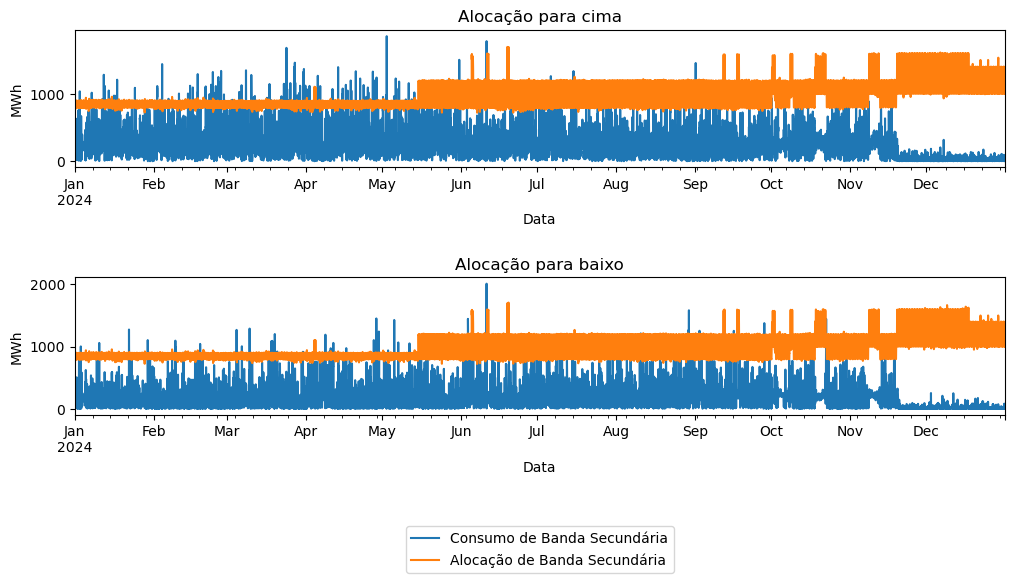
\includegraphics[width=\textwidth]{plots/benchmark_alocacoes_validacao.png}
    \caption{Série Temporal dos dados de Benchmark c/ consumo real}
    \label{fig:benchmarktimeseries}
\end{figure}

Imediatamente podemos verificar que o método para prever a energia necessária actualmente está dentro de um espectro limitado de valores, sendo que esses valores estão perto dos valores de ponta na alocação para cima, e perto dos valores médios na alocação para baixo.\\
Isto deve-se ao facto de ser uma função fixa, baseado no dia em questão. Notamos também que a meio de 2022 houve uma mudança dessa função que limitou os alcances tornando os valores mais elevados. Devido à guerra na Ucrânia e à forte incerteza que esta trouxe aos mercados de eletricidade por causa da crise de gás na Europa, que aumentou significativamente o preço deste recurso e levou à adaptação dos consumidores e países, a Red Eléctrica de España (\gls{REE}) aumentou as necessidades de reserva secundária para responder a esta incerteza.\\
Do ponto de visto de dados faz sentido para diminuir a quantidade  de vezes em que não é alocada energia suficiente.\\
Mas o mais importante a notar é a forma estática destes métodos, dado a natureza flutuante dos da energia necessária este método apresenta frequentemente um erro grande.\\
Podemos ver em pormenor analisando algumas janelas temporais dentro do período de validação. Vendo o melhor e pior resultado, em termos de erro absoluto, em janelas temporais de ano, mês, semana e dia.\\


\begin{figure}[H]
    \centering
    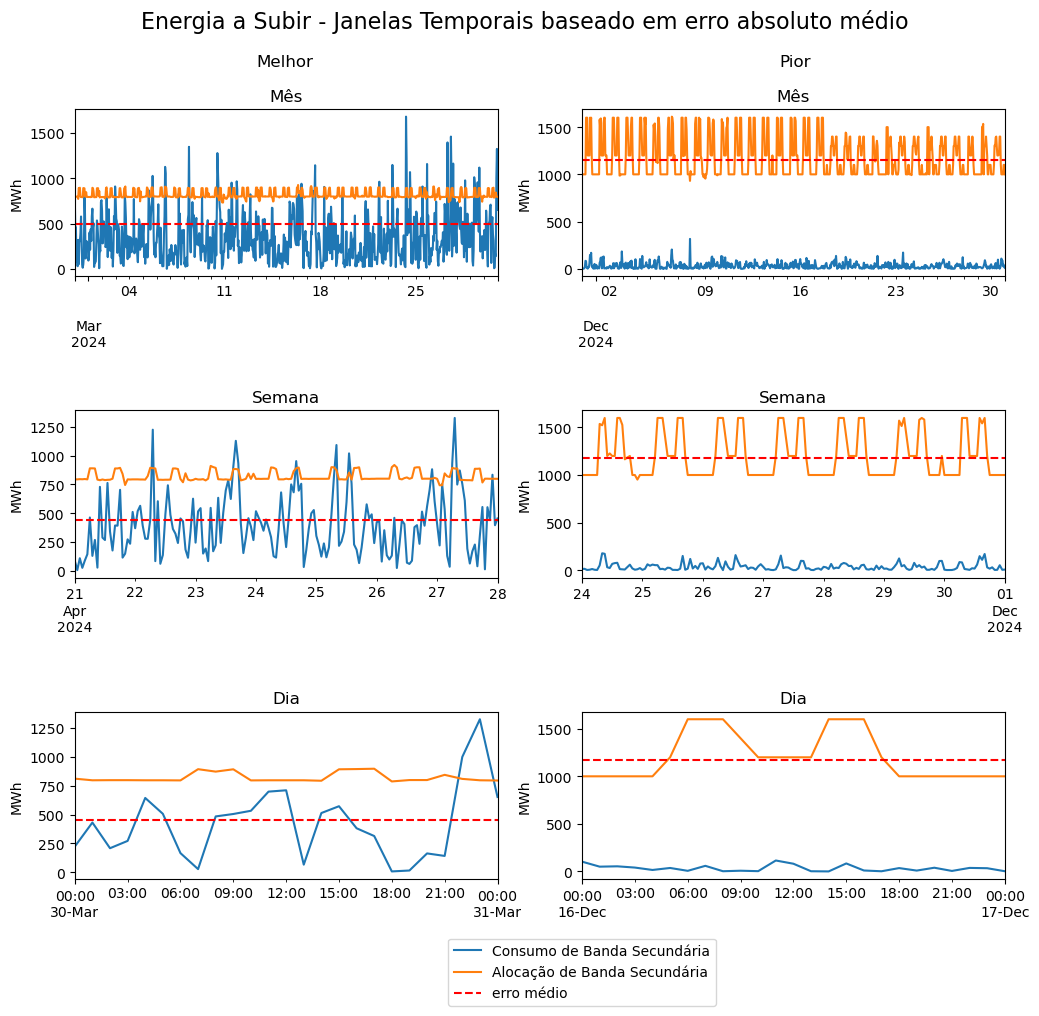
\includegraphics[width=\textwidth]{plots/alocacoes_temporais_upward_dataset.png}
    \caption{Janelas temporais de benchmark energia a subir}
    \label{fig:benchmarktimewindowsup}
\end{figure}


\begin{figure}[H]
    \centering
    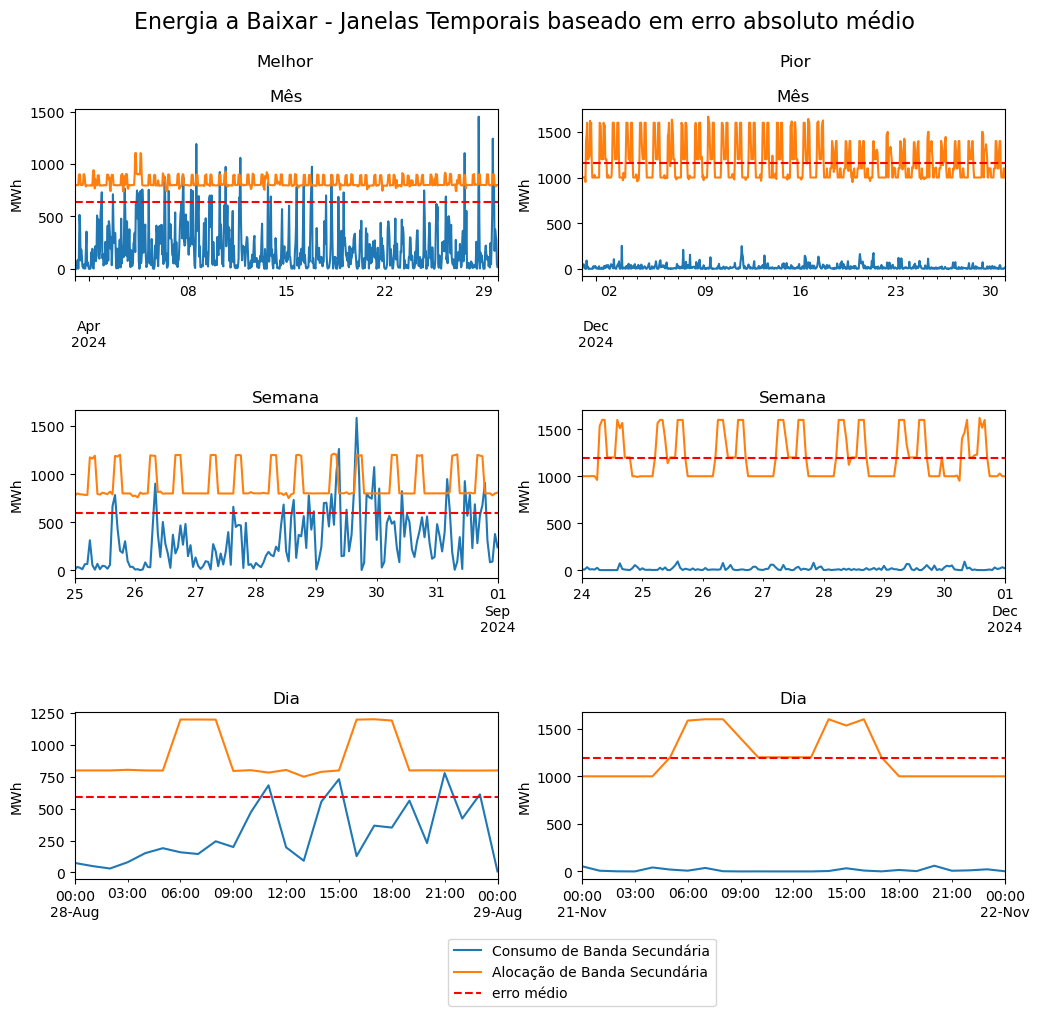
\includegraphics[width=\textwidth]{plots/alocacoes_temporais_downward_dataset.png}
    \caption{Janelas temporais de benchmark energia a descer}
    \label{fig:benchmarktimewindowsdown}
\end{figure}

Dentro destas janelas temporais conseguimos ter melhor a percepção da natureza estática deste modelo actual, e quão longe está dos valores reais necessários.\\

Os resultados a querer melhorar são:\\
\begin{table}[H]
    \caption{Resultados métricas benchmark}    
    \resizebox{\linewidth}{!}{\begin{table}[H] 
    \caption{This is a table caption. Tables should be placed in the main text near to the first time they are~cited.\label{tab1}}
    \newcolumntype{C}{>{\centering\arraybackslash}X}
    \begin{tabularx}{\textwidth}{CCCCC}
    \toprule
    & \textbf{RMSE}	& \textbf{SAE}	& \textbf{AllocF} & \textbf{AllocD}\\
    \midrule
    Up Allocation (MW) & 536.55 & 17357826.75 & 152679.00 & 17205147.75 \\
    Down Allocation (MW) & 408.99 & 12981575.55 & 479191.60 & 12502383.95 \\
        \bottomrule
    \end{tabularx}
    % \noindent{\footnotesize{\textsuperscript{1} Tables may have a footer.}}
\end{table}

}
    \label{tab:benchmarkmetrics}
    \end{table}

As correlações entre o método actual e a energia consumida podem ser vistas na figura abaixo:\\


\begin{figure}[H]
    \centering
    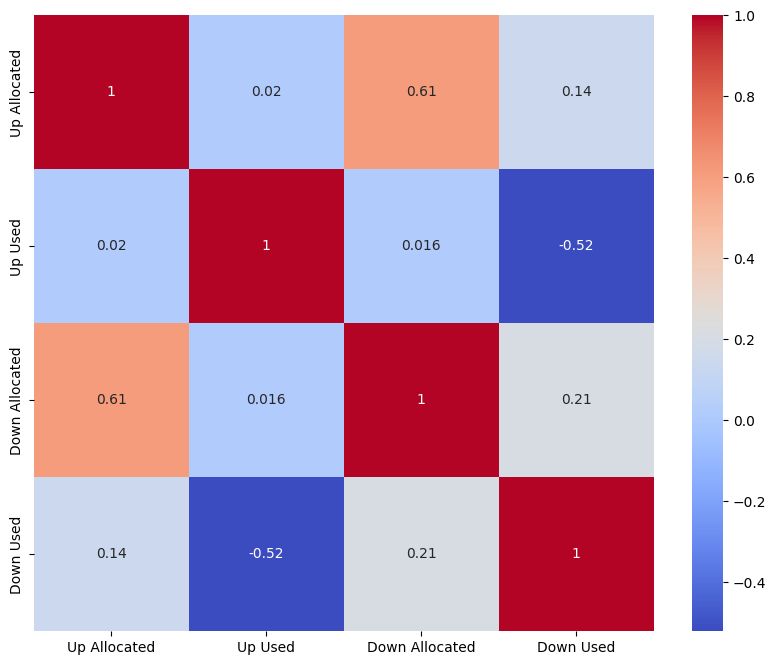
\includegraphics[width=\textwidth]{plots/correlation_heatmap_benchmark.png}
    \caption{Correlação entre benchmark e real}
    \label{fig:benchmarkcorr}
\end{figure}

% TODO: meter formula da previsão ENTO-e no capitulo estudo 2
As relações entres as energias alocadas são altas devido à natureza do \hyperref[]{método de previsão} enqanto que a correlação entre a energia alocada e a usada são bastante baixas com 21\% na alocaçao a descer e 2\% na alocação a subir.\\
O que não mostra uma ligaçao entre as alocações e a energia usada, mas apenas entre as energias alocadas.\\



